\section{Sets}
\subsection{Sets and Subsets}

A \textbf{set} is a collection of objects. Objects in a set are called \textbf{elements}.
Order does \underline{not} matter, and there are \underline{no} duplicates.

Roster notation:
\begin{align*}
  A & = \{2, 4, 6, 10\} \\
  B & = \{4, 6, 10, 2\} \\
  A & = B
\end{align*}

To show membership, use the \(\in\) symbol. For example, \(2 \in A\), while \(7 \not \in A\).
The empty set, which contains nothing, typically uses the \(\emptyset\) symbol, or \{\}.
Sets can be finite, or infinite. \textbf{Cardinality} of a set is the number of elements in a set.
For example, the cardinality of A is 4.
\begin{align*}
  \left\lvert A\right\rvert = 4
\end{align*}
Cardinality can be infinite. Consider the set of all the integers, \(\mathbb{Z}\). \(\left\lvert \mathbb{Z}\right\rvert = \infty\)

\begin{align*}
  \mathbb{N} & : \text{ set of natural numbers}                                         \\
             & = \{0, 1, 2, 3, \ldots\}                                                 \\
  \\
  \mathbb{Z} & : \text{ set of integers}                                                \\
             & = \{\ldots, -2, -1, 0, 1, 2, \ldots\}                                    \\
  \\
  \mathbb{Q} & : \text{ set of rational numbers}                                        \\
             & = \{x | x = \frac{a}{b} \text{ where } a, b \in \mathbb{Z}, b \not = 0\} \\
  \\
  \mathbb{R} & : \text{ set of real numbers}                                            \\
             & = \{x | x \text{ has a decimal representation}\}
\end{align*}

The subset operator is \(\subseteq\)
\begin{align*}
  A         & \subseteq B \text{  if } \forall x (x \in A \rightarrow x \in B) \\
  A         & \subseteq A \text{  is true for \underline{any} set}             \\
  \emptyset & \subseteq A \text{ is true for \underline{any} set}
\end{align*}

Sometimes it is easier to define a set by defining properties that all the elements have.
That is easy to do in \textbf{set builder notation}.
\begin{align*}
  A & = \{x \in S: P(x)\}, \text{ where \(S\) is another set}              \\
  C & = \{x \in \mathbb{Z}: 0 < x < 100 \text{ and } x \text{ is prime}\}. \\
  D & = \{x \in \mathbb{R}: \left\lvert x\right\rvert < 1\}
\end{align*}

The \textbf{Universal Set}, usually called 'U', is a set that contains all elements mentioned in a particular context.
For example, a discussion about certain types of real numbers, it would be understood that any element in the discussion
is a real number. Sets are often represented pictorially with \textbf{Venn Diagrams}.

\begin{center}
  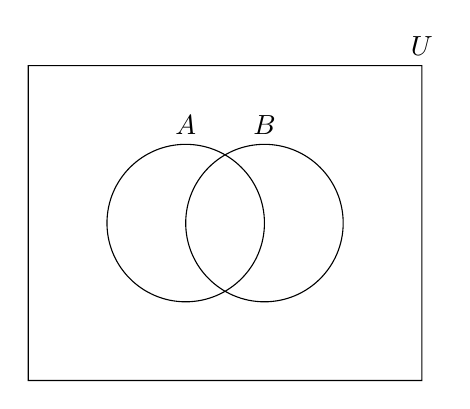
\begin{tikzpicture}[fill=white]
    \draw (0,0) circle (1) (0,1)  node [text=black,above] {$A$}
    (1,0) circle (1) (1,1)  node [text=black,above] {$B$}
    (-2,-2) rectangle (3,2) node [text=black,above] {$U$};
  \end{tikzpicture}
\end{center}

If \(A \subseteq B\) and there is an element of $B$ that is not an element of $A$, meaning \(A \not = B\),
then $A$ is a \textbf{proper subset} of $B$, denoted as \(A \subset B\). An important fact is that
\begin{center}
  \(\mathbb{N} \subset \mathbb{Z} \subset \mathbb{Q} \subset \mathbb{R}\)
\end{center}

\subsection{Sets of sets}
\subsection{Union and Intersection}
\subsection{More set operations}
\subsection{Set identities}
\subsection{Cartesian products}
\subsection{Partitions}